\documentclass[12pt]{article} % increase font size

%% Language and font encodings
\usepackage[english]{babel}
\usepackage[utf8x]{inputenc}
\usepackage[T1]{fontenc}
\usepackage{setspace}
\usepackage{titlesec}
\usepackage[affil-it]{authblk}  % advanced author info
\usepackage{graphicx}% Include figure files
\usepackage{listings} % syntax highlighting
\usepackage{xcolor}

\titlelabel{\thetitle.\quad} % Add a dot to section numbers
\newcommand\tab[1][1cm]{\hspace*{#1}} % create /tab command
\titleformat*{\section}{\large\bfseries} % shrink section titles
\setlength{\parindent}{0pt} % prevent auto-tab

%% Sets page size and margins
\usepackage[a4paper,top=2.5cm,bottom=3cm,left=2.5cm,right=2.5cm,marginparwidth=1.75cm]{geometry}

\lstdefinestyle{myJava}{
  language=Java,
  tabsize=3,
  basicstyle=\footnotesize,
  showspaces=false,
  showstringspaces=false,
  keywordstyle=\color{green!40!black},
  identifierstyle=\color{blue}
}


\title{Artificial Neural Network Training Through Simulated Natural Selection}
\author{Kyle D. Rocha-Brownell}
\affil{Departments of Physics and Computer Science}
\affil{California State University, Chico}
\date{}

\begin{document}

\maketitle
\doublespacing
\vspace{-5ex}
\begin{abstract}
An environment programmed to train Artificial Neural Networks (ANNs) through simulated natural selection is presented.  Numerous objects with independent ANNs interact with each other, competing for simulated limited resources.  A description of the process and technologies used is presented, followed with a discussion of the results.
\end{abstract}


\section{Artificial Neural Networks}
Artificial Neural Networks (ANNs) are an effective implementation of Artificial Intelligence (AI) which can be trained to accomplish specific tasks.  They are computational structures that take a series of numeric inputs, perform mathematical operations on them, and provide a series of output values.  The mathematical operations, called "activation functions," are independently carried out in each neuron. The results are then weighted by a unique value and sent to subsequent neurons, much like the firing of neurons in biological neural networks - brains. The ANN weights begin at random values, and are varied during training until the desired output is achieved.  See Figure 1 in the appendix for a visual representation of a single ANN.
\newline
\tab ANNs have been very successful in implementing AI where previous methods have failed.  They are particularly useful in areas where humans have traditionally outperformed computers, such as recognizing patterns.  Specific examples of this are facial recognition and handwriting recognition.


\section{Motivation}
The process of training an ANN involves providing feedback, often manually, to change the neuron weights until the desired output is achieved. One promising alternative avenue of research in the area of training ANNs is simulated natural selection, which falls under the broader category of Reinforcement Learning.  As long as an environment can be created in which successful ANNs thrive, and unsuccessful ones are destroyed automatically, training can be accomplished with little manual interaction.  To demonstrate the potential of this approach, an environment was created to train basic fight-or-flight intelligence into ANNs.


\section{Methods}
The Java programming language was used to implement an ANN in an attempt to "evolve" intelligence within a population of AI objects, referred to as individuals, through simulated natural selection.  The program output includes a visual simulation of the population as the individuals interact with each other in two dimensions (see Figure 2).  Each individual is represented as a colorful circle moving on a plane.  The program imposes a set of laws on the population that affect their condition, but on initialization of the simulation, each individual begins only with a randomly weighted ANN.
\newline
\tab The laws imposed by the program are essentially the rules for simple living creatures.  When multiple individuals are within a certain range, they will attempt to consume each other.  The value of the consumption (nutritionRatio) is given by the following function of their relative color:

\begin{minipage}{90em}
\begin{lstlisting}[style=myJava]
public double nutritionRatio(Blob otherBlob) { 
	double colorTaste = 
		( color.getRed()  / 255.0 * otherBlob.color.getGreen()/ 255.0
		+ color.getGreen()/ 255.0 * otherBlob.color.getBlue() / 255.0 
		+ color.getBlue() / 255.0 * otherBlob.color.getRed()  / 255.0 
		) / 3;
	return (colorTaste); 
} 
\end{lstlisting}
\end{minipage}

See Figure 3 for a qualitative description.  The purpose of this is to give each individual some preference toward what they consume.  They must also multiply (produce a new individual) once they have consumed a certain amount.  A newly created individual begins with an ANN weighted similarly to its parent, but with each weight randomly varied by a small percentage.  Their color is also varied slightly from that of the parent.  In theory, the individuals who have the most effective neural weights will survive to reproduce, and others will not.  As the generations pass, the ANNs should be increasingly effective at ensuring survival. 
\newline
\tab The inputs to the ANNs are essentially the “senses” of each individual.  They include the individual's own color and data on a number of other nearby individuals; specifically, their color and relative position in polar coordinates.  The output of the ANN is simply the desired direction of movement in radians.
\newline
\tab The success of an individual will be gauged based on its ability to survive.  Those who have produced the most offspring will be deemed most successful, as that indicates that they have successfully consumed many others, and have likely survived for a long period of time.


\section{Results}
After running for approximately 20 generations, ANNs with as few as 19 neurons were consistently weighted in a manner that attempted to keep their individuals "alive."  That is, the individuals moved toward those that they preferred to consume and stayed away from those that would consume them.  
\newline
\tab During some runs of the simulation, after a certain amount of time the entire population of individuals tended to be the same color, giving them little consumption value.  Many also utilized the strategy of avoiding interaction with all other individuals, regardless of their coloration.  Though these strategies do ensure survival, they do not exemplify the definition of success posited in the previous section.  Therefore, both tendencies were prevented in later runs by imposing an age limit on all individuals.  However, in all cases the age limit eventually resulted in total extinction.  To prevent extinction, a system was added to create new individuals with randomly weighted ANNs in order to keep the population above a certain value.


\section{Conclusion}
Though computationally expensive, simulated natural selection is a viable method for training ANNs where applicable.  This first implementation in Java was admittedly inefficient, in that the program ran in a largely serial manner.  Future implementations should be run on a parallel platform such as NVidia’s CUDA application programming interface.  This would provide a much faster simulation, resulting in more generations passing in a given time.
\newline
\tab The most challenging aspect of simulated natural selection is creating an environment that will train the ANNs in the desired manner.  Though a given environment may tend to generate successful ANNs, it may only do so at a certain time.  A balance must be achieved to assure that all ANNs remain consistently motivated in a way that results in proper training.

\newpage

\section{Appendix}


\begin{figure}[ht]
\centering
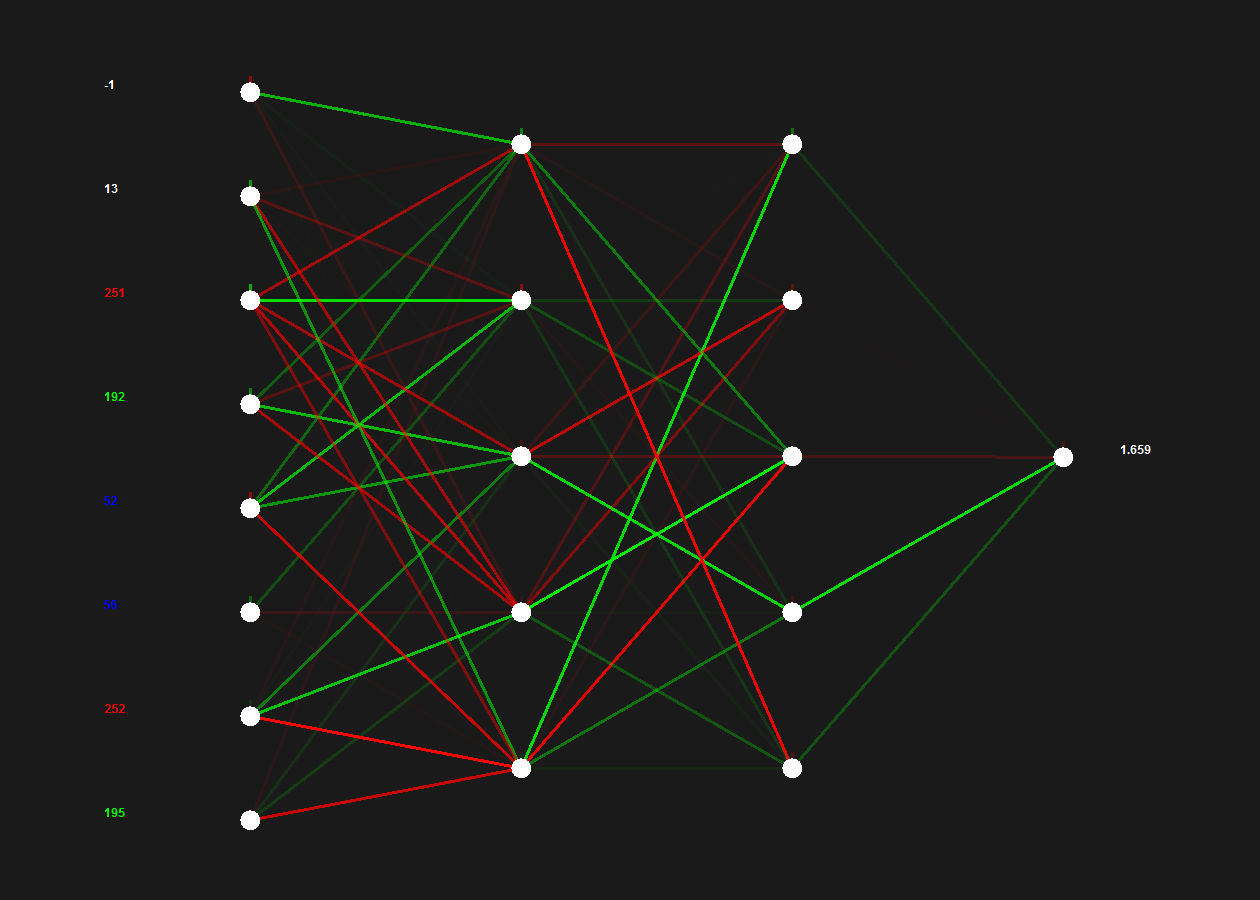
\includegraphics[width=0.55\textwidth]{ANN.png}
\caption{
A visual representation of an ANN taken from the simulation.  The numbers on the left are the numeric inputs to the network, and the number on the right is the output.  The brightness of the connecting line colors indicate the relative value of the weights between the white neurons (red weights are negative and green are positive).
\newline
\newline
}
\end{figure}


\begin{figure}[ht]
\centering
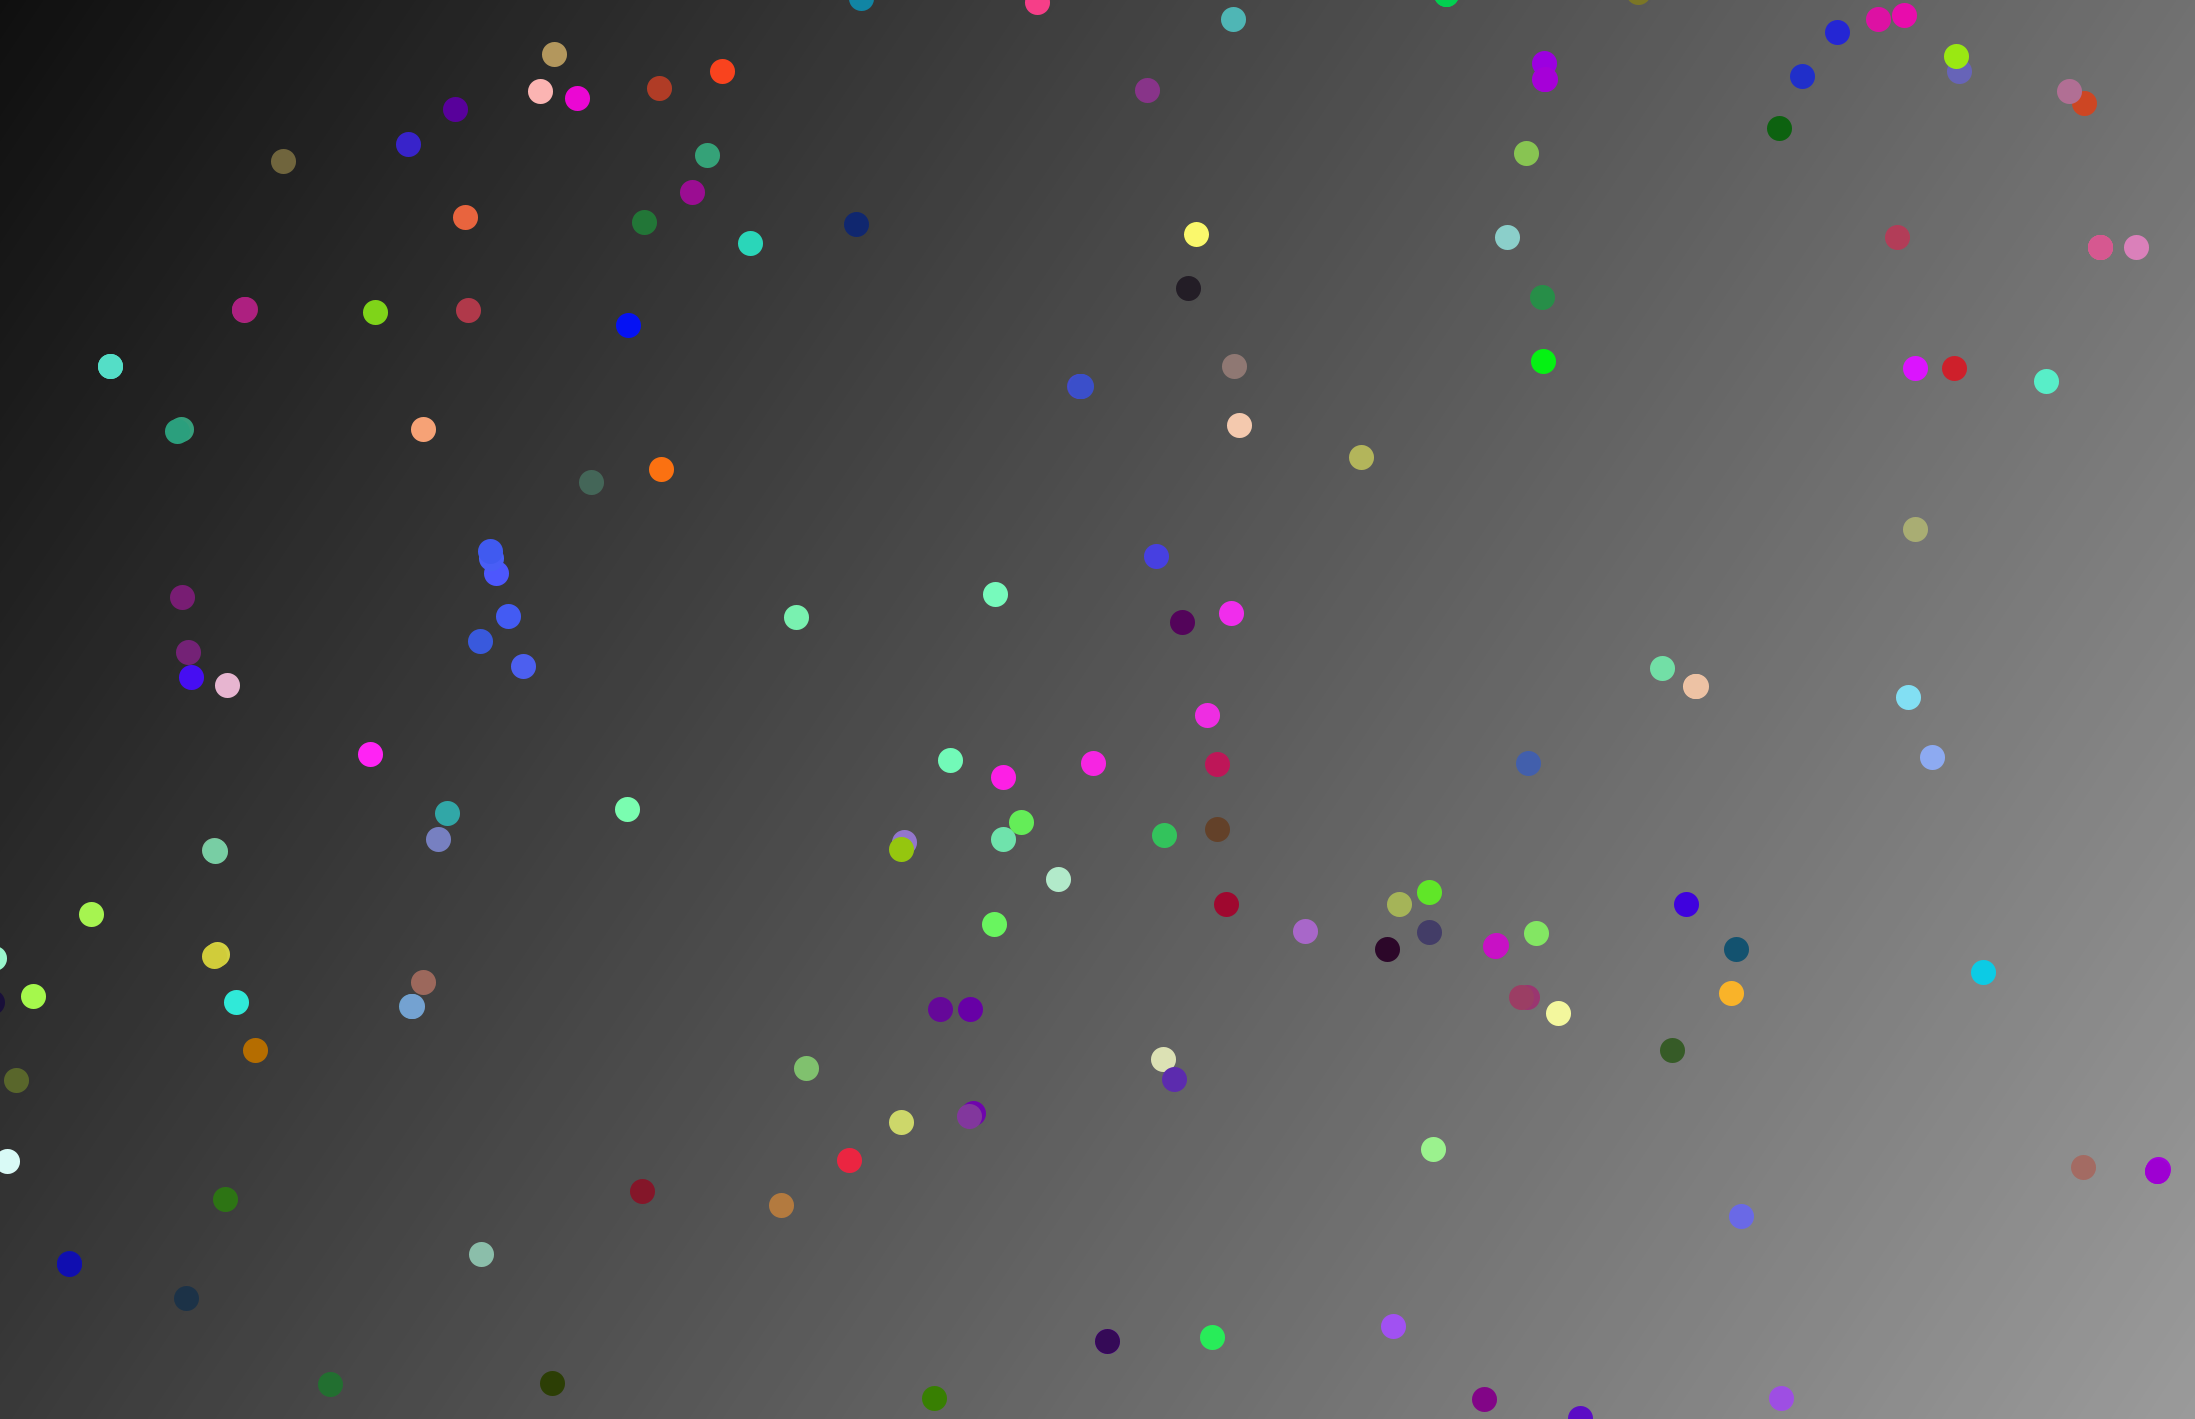
\includegraphics[width=0.65\textwidth]{population.png}
\caption{
A simulation frame of the population of different colored individuals interacting with each other. Each individual contains its own ANN.
}
\end{figure}


\begin{figure}[ht]
\centering
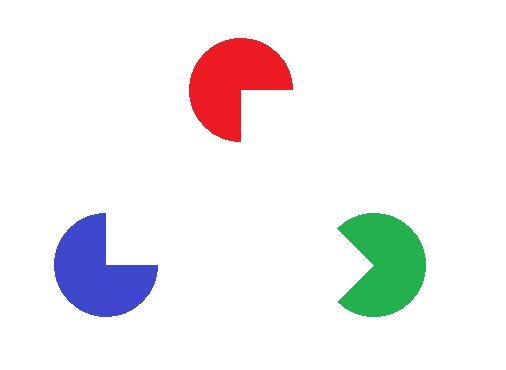
\includegraphics[width=0.7\textwidth]{diet.png}
\caption{
A visual description of the consumption preference that individuals have for one another.  For example, primarily green individuals can consume primarily blue individuals, but are consumed by primarily red individuals.
}
\end{figure}

\end{document}